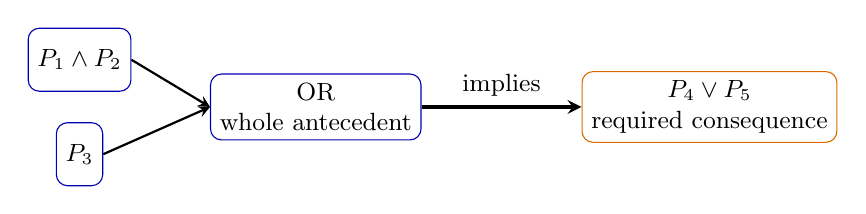
\begin{tikzpicture}[>=stealth,box/.style={draw,rounded corners,align=center,font=\small,minimum height=.8cm}]
\node[box,draw=blue!70!black](a)at(0,.6){$P_1\land P_2$};
\node[box,draw=blue!70!black](b)at(0,-.6){$P_3$};
\node[box,draw=blue!70!black](o)at(3,0){OR\\whole antecedent};
\node[box,draw=orange!85!black](r)at(8,0){$P_4\lor P_5$\\required consequence};
\draw[->,thick](a.east)--(o.west);\draw[->,thick](b.east)--(o.west);
\draw[->,very thick](o.east)--node[above,font=\small]{implies}(r.west);
\end{tikzpicture}
